\documentclass[reqno,12pt]{amsart}

\usepackage{tikz}
\usepackage{graphics,amssymb,amsmath}
\input cyracc.def
\font\tencyr=wncyr8
\def\cyr{\tencyr\cyracc}
\oddsidemargin 5.75mm
\evensidemargin 5.75mm
\textheight = 45\baselineskip
\textwidth 150mm
\newcommand{\shift}{\mbox{}\hspace{4.5mm}}
\newcommand{\fix}[1]{\mathit{fix}(#1)}
\newcommand{\lin}[1]{\bar v(#1)}
\newcommand{\free}[1]{\tilde v(#1)}
\newcommand{\fixl}[1]{\mathit{fix}^-(#1)}
\newcommand{\fitl}[1]{\mathit{fit}^-(#1)}
\newcommand{\fitg}[1]{\mathit{fit}^\vee(#1)}
\newcommand{\cut}[1]{\bar f(#1)}
\newcommand{\ff}{{\bar f}}
\newcommand{\vv}{{\bar v}}
\newcommand{\plin}[1]{\stackrel{=}{v}(#1)}
\newcommand{\pcute}[1]{\stackrel{=}{e}(#1)}
\newcommand{\fit}[1]{\mathit{fit}(#1)}
\newcommand{\fixx}[1]{\mathit{fix}^X(#1)}
\newcommand{\fitx}[1]{\mathit{fit}^X(#1)}
\newcommand{\foldn}[1]{{\sc Fold}}
\newcommand{\fold}[2]{{\sc Fold}}
\newcommand{\cross}[1]{\mathrm{cr}(#1)}
\newcommand{\reals}{\mathbb{R}}
\newcommand{\function}[2]{:#1 \rightarrow #2}
\newcommand{\of}[1]{\left( #1 \right)}
\newcommand{\setdef}[2]{\left\{ \hspace{0.5mm} #1 : \hspace{0.5mm} #2 \right\}}
\newcommand{\refeq}[1]{(\ref{eq:#1})}
\newcommand{\hide}[1]{}
\newcommand{\edit}[1]{}


\newtheorem{theorem}{Theorem}[section]
\newtheorem{lemma}[theorem]{Lemma}
\newtheorem{example}[theorem]{Example}
\newtheorem{question}[theorem]{Question}
\newtheorem{corollary}[theorem]{Corollary}
\newtheorem{remark}[theorem]{Remark}

\newenvironment{proofof}[1]{\par\smallbreak\noindent{\it Proof~of~#1.}}{\unskip\nobreak\hfill \qed \par\medbreak}
\newcommand{\Case}[2]{\smallskip\par{\it Case #1:\/ #2}}
\newcommand{\Subcase}[2]{\smallskip\par{\it Subcase #1:\/ #2}}
\newenvironment{bfenumerate}{\renewcommand{\labelenumi}{{\bf\theenumi.}}\renewcommand{\labelenumii}{{\bf(\theenumii)}}\begin{enumerate}}{\end{enumerate}}
\newcounter{oq}
\newcommand{\que}{\refstepcounter{oq}\par{\sc \theoq.}~}
\title{On collinear sets in straight line drawings}

\author{Alexander Ravsky\,}\thanks{\,Institute for Applied Problems of Mechanics and Mathematics,
Naukova St.\ 3-{\cyr B}, Lviv 79060, Ukraine.}

\author{Oleg Verbitsky\,}\thanks{\,Current address: Humboldt-Universit\"at zu Berlin,
Institut f\"ur Informatik, Unter den Linden 6,
D-10099 Berlin. Supported by the Alexander von Humboldt Foundation.}


\date{}

\begin{document} 


\begin{abstract}
We consider straight line drawings of a planar graph  with possible edge crossings.
The \emph{untangling problem} is to eliminate all edge crossings by moving as few
vertices as possible to new positions.
Let  denote the maximum number of vertices that can be left fixed
in the worst case.
In the \emph{allocation problem}, we are given
a planar graph  on  vertices together with an -point set 
in the plane and have to draw  without edge crossings so that
as many vertices as possible are located in .
Let  denote the maximum number of points fitting this purpose
in the worst case.
As , we are interested in upper bounds for the latter
and lower bounds for the former parameter.

For each , we construct an infinite sequence of graphs 
with ,
where  is a known graph-theoretic constant, namely the shortness
exponent for the class of cubic polyhedral graphs. 
To the best of our knowledge, this is the first example of graphs
with .
On the other hand, we prove that  for all  with tree-width
at most 2. This extends the lower bound obtained by 
Goaoc et al.\ [{\it Discrete and Computational Geometry\/} 42:542--569 (2009)]
for outerplanar graphs.

Our upper bound for  is based on the fact that the constructed graphs
can have only few collinear vertices in any crossing-free drawing.
To prove the lower bound for , we show that graphs of tree-width 2
admit drawings that have large sets of collinear vertices with some additional
special properties.
\end{abstract}

\maketitle
\markleft{\sc ALEXANDER RAVSKY and OLEG VERBITSKY}

\section{Introduction}


\subsection{Basic definitions}

Let  be a planar graph. The vertex set of  will be denoted by .
The letter  will be reserved to always denote the number of vertices in .
By a \emph{drawing} of  we mean an arbitrary injective map
.
The points in  will be referred to as \emph{vertices} of the drawing.
For an edge  of ,
the segment with endpoints  and  will be referred to as an \emph{edge}
of the drawing. Thus, we always consider \emph{straight-line} drawings.
It is quite possible that in  we encounter edge crossings and even overlaps.
A drawing is \emph{plane} (or \emph{crossing-free}) if this does not happen.


Given a drawing  of  , define

Given an -point set  in the plane, let

Furthermore, we define

In other words,  is the maximum number of vertices
which can be fixed in any drawing of  while \emph{untangling} it.

Given an -point set , consider now a related parameter

In words, if we want to draw  allocating its vertices at points of , then
 tells us how many points of  can fit for this purpose.
To analyze the \emph{allocation} problem in the worst case, we define

Note that .
It follows that  and, therefore,
.


\subsection{Known results on the untangling problem}

No efficient way for evaluating the parameter  is known.
Note that computing  is NP-hard \cite{merged,Ver}.
Essential efforts are needed to estimate  even for cycles, for which
we know bounds

due to, respectively, Cibulka \cite{Cib} and Pach and Tardos \cite{PTa}.
In the general case Bose et al.~\cite{Bose} establish a lower bound

A better bound
 
is proved for all trees (Bose et al.~\cite{Bose}, Goaoc et al.~\cite{merged}) 
and, more generally, outerplanar graphs (Goaoc et al.~\cite{merged}, cf.\ Corollary \ref{cor:outer} below). 

On the other hand, \cite{Bose,merged,KPRSV} provide examples of planar
graphs (even acyclic ones) with 

In particular, for the fan graphs  we have

see \cite{KPRSV}.
Cibulka \cite{Cib} establishes some general upper bounds, namely 
for graphs whose maximum degree and diameter are bounded by a logarithmic function and
 for 3-connected graphs.


\subsection{Known results on the allocation problem}

The question whether or not  has been studied in the literature,
especially for  in general position.
If  is in convex position, any triangulation on  is outerplanar.
By this reason,  for all non-outerplanar graphs  and all
sets  in convex position.
On the other hand, in \cite{GritzmannMPP91} it is proved that
 for all outerplanar  and all  in general position.
Other results and references on this subject can be found, e.g., in~\cite{GarciaHHTV09}.

It is known that there are 
unlabeled planar graphs with  vertices \cite{GimenezN09}, while a set of  points in convex position
admits no more than  plain drawings \cite{FlajoletN99}. Combining the two results, we see
that, if  is in convex position, then  for almost all planar~.



\subsection{Our present contribution}


We aim at proving upper bounds for  and lower bounds for .
Our approach to both problems is based on analysis of collinear sets of vertices
in straight line graph drawings. We show the relevance of the following questions.
How many collinear vertices can occur in a plane drawing of a graph ?
If there is a large collinear set, which useful features can it have?

Suppose that  is a crossing-free drawing of a graph .
A set of vertices  in  is \emph{collinear} if all of them
lie on a line . By a \emph{conformal displacement} of 
we mean a relocation  preserving the relative order in which
the vertices in  lie in . We call  \emph{free} if every
conformal displacement  is extendable to a mapping
 so that  is a crossing-free
drawing of  (i.e., whenever we shift vertices in  along  without breaking
their relative order, then all edge crossings that may arise can be eliminated by subsequently
moving the vertices in ).
Let  denote the maximum size of a collinear set in  and
 the maximum size of a free collinear set in .
Define

Obviously, . These parameters have a direct relation to  and , namely

The latter inequality follows immediately from the definitions. The first
inequality is proved as Theorem \ref{thm:fixfree} below.

In Section \ref{s:lin} we construct,
for each , an infinite sequence of graphs with 
where  is a known graph-theoretic constant, namely the shortness
exponent for the class of cubic polyhedral graphs (see Section \ref{s:prel} for the definition). 
To the best of our knowledge, this gives us the first example of graphs with
. While the known upper bounds \refeq{fixupper} for  are still better,
note that the problems of bounding  and  from above are inequivalent.
The two parameters can be far away from one another: 
for example, in contrast with \refeq{fixxFn} we have  for any~.


By the lower bound in \refeq{freefixlin}, we have  whenever
. Therefore, identification of classes of planar graphs with linear 
is of big interest. In Section \ref{s:free} we show that
 for every outerplanar graph .
This gives us another proof of the bound  proved for
outerplanar graphs by Goaoc et al.~\cite{merged}\footnote{A preliminary version of \cite{merged} gave a somewhat worse bound of .
An improvement to  was made in the early version of the present paper
independently of~\cite{merged}.}.

Furthermore, we consider the broader class of graphs with tree-width at most 2.
It coincides with the class of partial 2-trees and contains also all series-parallel graphs
(see, e.g.\ \cite[Sect.\ 8.3]{Bodlaender98}). For any graph  in this class, we prove
that  and, therefore, .
The proof of this result takes Section \ref{s:2trees}.
Note that the sublinear upper bound for  is established in Section \ref{s:lin}
for a sequence of graphs whose tree-width is bounded by a constant.
We conclude with the discussion of open problems in Section~\ref{s:open}.




\section{Preliminaries}\label{s:prel}

Given a planar graph , we denote the number of vertices, edges,
and faces in it, respectively, by , , and . The latter number
does not depend on a particular plane embedding of  and hence is well defined.
Moreover, for connected  we have

by Euler's formula. 

A graph is \emph{-connected} if it has more than  vertices and 
stays connected after removal of any  vertices. 
3-connected planar graphs are called \emph{polyhedral}
as, according to Steinitz's theorem, 
these graphs are exactly the 1-skeletons of convex polyhedra.
By Whitney's theorem, all plane embeddings of a polyhedral
graph  are equivalent, that is, obtainable from one another by a plane homeomorphism
up to the choice of outer face. In particular, the set of facial cycles (i.e.,
boundaries of faces) of  does not depend on a particular plane embedding.

A planar graph  is \emph{maximal} if adding an edge between any two 
non-adjacent vertices of  violates planarity. Maximal planar graphs 
on more than 3 vertices are
3-connected. Clearly, all facial cycles in such graphs have length 3.
By this reason maximal planar graphs are also called \emph{triangulations}.
Note that for every triangulation  we have
.
Combined with \refeq{euler}, this gives us


The \emph{dual} of a polyhedral graph  is a graph  whose
vertices are the faces of  (represented by their facial cycles).
Two faces are adjacent in  iff they share a common edge.
 is also a polyhedral graph. If we consider , we obtain
a graph isomorphic to . In a \emph{cubic} graph every vertex is
incident to exactly 3 edges. As easily seen, the dual of a triangulation
is a cubic graph. Conversely, the dual of any cubic polyhedral graph 
is a triangulation.

The \emph{circumference} of a graph , denoted by , is the
length of a longest cycle in . The \emph{shortness exponent}
of a class of graphs  is the limit inferior of quotients 
over all . Let  denote the shortness exponent
for the class of cubic polyhedral graphs. It is known that

(see \cite{BilinskiJMY11} for the lower bound and \cite[Theorem 7(iv)]{GWa} for the upper bound).




\section{Graphs with small collinear sets}\label{s:lin}

We here construct a sequence of triangulations  with .
For our analysis we will need another parameter of a straight line drawing.
Given a crossing-free drawing  of a graph ,
let  denote the maximum number of collinear points in the plane
such that each of them is an inner point of some face of 
and no two of them are in the same face. Let .
In other words,  is equal to the maximum number of faces in
some straight line drawing of  whose interiors can be cut by a line.
Further on, saying that a line \emph{cuts} a face, we mean that the line
intersects the interior of this face.

For the triangulations constructed below, we will show that 
is small with respect to  because  is small with respect
to  (though we do not know any relation between  and  in general). 
Our construction can be thought of as a recursive procedure
for essentially decreasing the ratio  at each recursion step
provided that we initially have .

\begin{figure}
\centerline{\scalebox{0.85}{\includegraphics{fromK4.eps}}}
\caption{An example of the construction: , , .}
\label{fig:fromK4}
\end{figure}

Starting from an arbitrary triangulation  with at least 4 vertices, 
we recursively define 
a sequence of triangulations . To define , we will
describe a spherical drawing  of this graph. Let  be
an arbitrary drawing of  on a sphere. Furthermore, 
is obtained from  by triangulating each face of  so
that this triangulation is isomorphic to . An example is shown
on Fig.~\ref{fig:fromK4}. In general, upgrading  to 
can be done in different ways, that may lead to non-isomorphic versions
of . We make an arbitrary choice and fix the result.


\begin{lemma}\label{lem:Gk}
Denote , , and .
\begin{bfenumerate}
\item
.
\item
.
\item
, where  is a constant depending only on~.
\end{bfenumerate}
\end{lemma}



\begin{proof}
The first part follows from the obvious recurrence

We have to prove the other two parts.

Consider an arbitrary crossing-free straight line drawing  of .
Recall that, by construction,  is a chain of subgraphs of  with

Let  be the part of  which is a drawing of the subgraph .
By the Whitney theorem,  can be obtained from  (the spherical
drawing defining ) by an appropriate stereographic projection of the sphere
to the plane combined with a homeomorphism of the plane onto itself.
It follows that, like  and , drawings  and 
have the following property: the restriction of  to any face of 
is a drawing of .
Given a face  of , the restriction of  to  (i.e., a plane
graph isomorphic to ) will be denoted by . 

Consider now an arbitrary line . Let  denote the number of faces
in  cut by . By definition, we have

For each , we have 
1mm]
\ff_i(\ff-1)&\mathrm{if}&\ff_i>1.
\end{array}
\right.
\label{eq:need}
\ff_i\le\ff(\ff-1)^{i-1}

\vv_1\le v-2

\vv_i\le\ff_{i-1}(v-3).
\label{eq:vv}
\vv\le(v-2)+(v-3)\sum_{i=1}^{k-1}\ff_i\le\frac{(v-3)\ff}{\ff-2}(\ff-1)^{k-1},

(\ff-1)^{k-1}=(f-1)^{\alpha(k-1)}<(2/f)^\alpha\, v(G_k)^\alpha.
\cut G\le c(G^*).
\plin G=\max_{\pi,\ell}\plin{\pi,\ell},

\pcute G=\max_{\pi,\ell}\pcute{\pi,\ell},
\label{eq:fixfixl}
\fix G=\fixl G.
-6.5mm]
\begin{itemize}
\item
draw  as ;
\item
choose three points , , and  inside  specifying a subfold of
this triangle;
\item
designate roots , , and  in 2-trees  , , and 
respectively (if any of these 2-trees is empty, this branch of the procedure terminates);
\item
invoke\\
\fold{}{G_{ab,c},abc',ABC'}, 
\fold{}{G_{ac,b},ab'c,AB'C}, and  
\fold{}{G_{bc,a},a'bc,A'BC}\\
(note that the three subroutines can be executed independently in parallel).
\end{itemize}

\smallskip

It is clear that \fold{}{G,abc,ABC} produces a drawing of  with outer face .
A drawing of  is called \emph{folded} if it can be obtained as the output of \fold{}{G,abc,ABC}.

Note that the described procedure is nondeterministic as we have a lot of freedom
in choosing points  and we can also have a choice of vertices .
We now introduce some notions allowing us to specify any particular computational
path of \foldn{}.

Any subfold of a geometric triangle  specified by points 
will be called a \emph{depth-1 subfold} of , and the triangles
, , and  will be referred to as its triangular faces
(the outer face, which is also triangular, is not taken into account).
A \emph{depth- subfold} of  is obtained from any depth- subfold
by subfolding each of its  triangular faces (thereby increasing
the number of triangular faces to ), see Fig.~\ref{fig:subfolds}.

\begin{figure}
\centering
 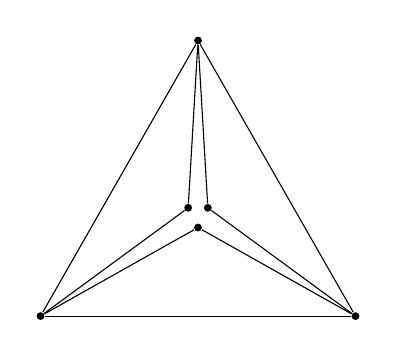
\begin{tikzpicture}[every node/.style={circle,fill,inner sep=1pt}]
  \path[scale=.25] (0,0) node[label=left:] (a)   {}
                 (16,0) node[label=right:] (b)   {} edge (a)
             (8,14) node[label=above:] (c)   {} edge (a) edge (b)
             (8,4.5) node[label=below:] (z)   {} edge (a) edge (b)
                 (7.5,5.5) node[label=above left:] (y) {} edge (a) edge (c)
               (8.5,5.5) node[label=above right:] (x)   {} edge (b) edge (c);
 \end{tikzpicture}
\qquad\qquad
 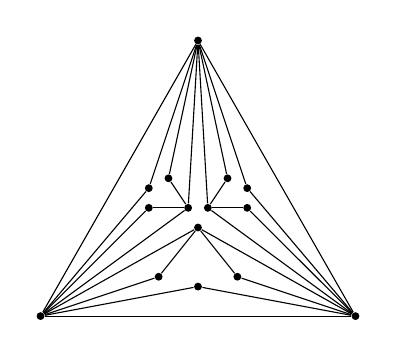
\begin{tikzpicture}[every node/.style={circle,fill,inner sep=1pt}]
  \path[scale=.25] (0,0) node[label=left:] (a)   {}
                 (16,0) node[label=right:] (b)   {} edge (a)
             (8,14) node[label=above:] (c)   {} edge (a) edge (b)
             (8,4.5) node (z)   {} edge (a) edge (b)
                 (7.5,5.5) node (y) {} edge (a) edge (c)
               (8.5,5.5) node (x)   {} edge (b) edge (c)
               (5.5,6.5) node (ac)   {} edge (a) edge (c)
               (6.5,7) node (cy)   {} edge (c) edge (y)
               (5.5,5.5) node (ay)   {} edge (a) edge (y)
               (9.5,7) node (xc)   {} edge (x) edge (c)
               (10.5,6.5) node (bc)   {} edge (b) edge (c)
               (10.5,5.5) node (xb)   {} edge (x) edge (b)
               (6,2) node (az)   {} edge (a) edge (z)
               (8,1.5) node (ab)   {} edge (a) edge (b)
               (10,2) node (bz)   {} edge (b) edge (z);
 \end{tikzpicture}
\caption{Subfolds of depth 1 and 2.}
\label{fig:subfolds}
\end{figure}

Given a 2-tree , let  be a tree with  rooted at .
Specification of a root determines the standard parent-child relation on .
We call  a \emph{subrooting tree} for  if every  has at most
three children and those are of the form , ,  for some .

Note that removal of the root  from  splits it into three subtrees
, , and  (some may be empty) such that , 
, and .
A similar fact holds true for any rooted subtree of 
(a rooted subtree is formed by its root  and all descendants of ).
This observation makes evident that each computational path of \fold{}{G,abc,ABC}
is determined by a subrooting tree  rooted at  and a depth- subfold 
of the triangle  (where  is equal to the height of ):
whenever the subroutine \fold{}{H,xyz,XYZ} is invoked for some 2-subtree  of ,
we choose the vertices  and the points  so that
, ,  are the children of  in , and
the geometric triangles , ,  form the subfold of  in 
(more precisely, in the fragment of  of the corresponding depth).
We will denote this path of the procedure \fold{}{G,abc,ABC} by \fold{}{R,S}.


Our goal is now to establish the following fact.

\begin{lemma}\label{lem:foldfree}
Every collinear set of vertices in a folded drawing is free.
\end{lemma}

We will derive Lemma \ref{lem:foldfree} from an elementary geometric fact
stated below as Lemma \ref{lem:foldfree2},
but first we make a few useful observations and introduce some technical notions.

Note that a depth- subfold is, in a sense, unique and rigid.
More precisely, any two subfolds of the same depth are equivalent up to homeomorphisms
of the plane
(as usually, it is supposed that a homeomorphism takes vertices of geometric graphs
to vertices and edges to edges). Moreover, if  is a depth- subfold of a triangle 
and a homeomorphism  takes  onto itself and fixes the vertices , , and 
(i.e.,  etc.), then  fixes every vertex of .
It follows that, once we identified the vertices of the triangle by the labels
, , and , each other vertex  of  can be identified by a \emph{canonical label} . 
Formally, a \emph{canonical labeling} of a depth- subfold  is an injective map ,
where a set of labels  contains the labels , , and  that are assigned to the vertices
of the outer triangle, such that any homeomorphism between two subfolds respecting the labels 
must respect the labels of all vertices.



A canonical labeling can be defined explicitly in many, essentially equivalent, ways.
To be specific, we can fix the following definition.
Let  be a depth- subfold of a triangle  obtained by a sequence
, where  is obtained from  by subfolding
each inner triangular face. Note that the sequence  is reconstructible
from . For example, the vertex  that is adjacent to  and  in 
is determined by the condition that  is the second largest triangle in
the inclusion-chain of triangles in  containing .
Now, we inductively extend the canonical labeling  from  to 
as follows:
if  is a triangular face of  and 
(hence ), then .

Furthermore, let  be a line such that no edge of  lies on it.
By  we will denote the set of common points of  and ,
consisting of the vertices of  lying on  and the points of intersection
of  with edges of . In addition to the canonical labeling of the vertices
of , we label each intersection point of  with an edge  of 
by . This allows us to define the \emph{intersection pattern}
of  and  to be the sequence of the labels of all points in 
as they appear along  (thus, this sequence is defined up to reversal).

Given two triangles  and , we will identify the matching vertex names,
that is,  and ,  and , and  and .

\begin{lemma}\label{lem:foldfree2}
Suppose that a line  intersects a triangle  in at least 2 points
and the same is true for a line  and a triangle .
Moreover, let  and  have the same intersection
pattern (for example, if  passes through  and crosses , then
 passes through  and crosses ).
Consider an arbitrary depth- subfold  of  and an arbitrary
set of points  within  such that
 and .
Then there exists a depth- subfold  of  such that
 and, moreover,  has the same intersection pattern
as .
\end{lemma}

\begin{proof}
We proceed by induction on . The base step of  is a trivial
geometric graph, see Fig.~\ref{fig:basecase}.
\begin{figure}
\centering
 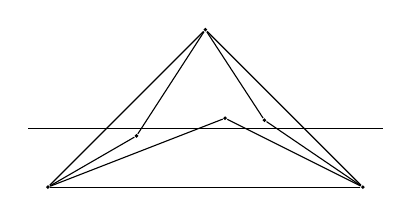
\begin{tikzpicture}[scale=.5,every node/.style={circle,fill,inner sep=.5pt}]
\draw (-0.5,1.5) -- (8.5,1.5);
  \path (0,0) node (a)   {}
                 (8,0) node (b)   {} edge (a)
             (4,4) node (c)   {} edge (a) edge (b)
             (4.5,1.75) node (ab)   {} edge (a) edge (b)
             (2.25,1.3) node (ac)   {} edge (a) edge (c)
             (5.5,1.7) node (bc)   {} edge (b) edge (c);
 \end{tikzpicture}
\hfill
 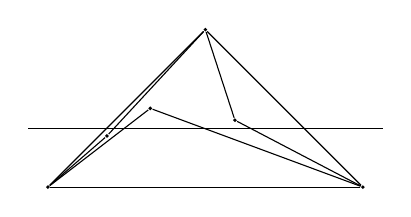
\begin{tikzpicture}[scale=.5,every node/.style={circle,fill,inner sep=.5pt}]
\draw (-0.5,1.5) -- (8.5,1.5);
  \path (0,0) node (a)   {}
                 (8,0) node (b)   {} edge (a)
             (4,4) node (c)   {} edge (a) edge (b)
             (2.6,2) node (ab)   {} edge (a) edge (b)
             (1.5,1.3) node (ac)   {} edge (a) edge (c)
             (4.75,1.7) node (bc)   {} edge (b) edge (c);
 \end{tikzpicture}
\hfill
 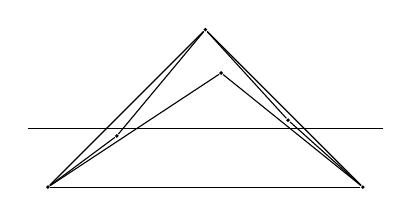
\begin{tikzpicture}[scale=.5,every node/.style={circle,fill,inner sep=.5pt}]
\draw (-0.5,1.5) -- (8.5,1.5);
  \path (0,0) node (a)   {}
                 (8,0) node (b)   {} edge (a)
             (4,4) node (c)   {} edge (a) edge (b)
             (4.4,2.9) node (ab)   {} edge (a) edge (b)
             (1.75,1.3) node (ac)   {} edge (a) edge (c)
             (6.1,1.7) node (bc)   {} edge (b) edge (c);
 \end{tikzpicture}
\caption{Base case in the proof of Lemma \protect\ref{lem:foldfree2}}
\label{fig:basecase}
\end{figure}
Suppose that . Then  is obtained from a depth-1 subfold  of 
by depth- subfolding each of its three triangular faces. Label
the points of  according to the intersection pattern of .
Let  consist of the points whose labels appear in .
Since the lemma is true in the base case, there is a subfold  of 
such that  and the intersection pattern of 
agrees with the labeling of .
Let  be the triangular faces of  and 
the corresponding triangular faces of .
For each , let  be the segment of  inside 
(it may be empty for some ). There remains to apply the induction hypothesis
to the lines  and , the triangles bounding  and ,
the depth- subfold of  induced by , and the point set ,
for each .
\end{proof}


\begin{proofof}{Lemma \ref{lem:foldfree}}
Given a folded drawing  and a line , we have to show that
 is free. Let  be the boundary of the outer face of .
It suffices to consider the case when  is a depth- subfold of ,
for some  (completing , if necessary, we will prove even a stronger fact).
Using the notion of a canonical labeling, our task can be stated as follows:
Given an arbitrary set  of  points on a line ,
we have to find a depth- subfold  of some triangle 
such that  and the intersection patterns of 
and  agree on  and .
The solvability of this task follows from Lemma~\ref{lem:foldfree2}.
\end{proofof}


\subsection{Folded drawings with many collinear leaf vertices}\label{ss:fold1}

Let  be a 2-tree. We will call  a \emph{leaf vertex} 
if it has degree 2. The two edges emanating from  will be referred to
as \emph{leaf edges}.
A triangle containing a leaf vertex will be called a \emph{leaf triangle}. 
The number of leaf triangles in  
will be denoted by . 
Our nearest goal is to show that there is a folded drawing of 
with at least  collinear leaf vertices.
The graph all whose triangles share an edge can be excluded from
consideration, as it can be drawn with all leaf vertices on a line.
This is the only case when a graph has only leaf triangles.
In the sequel we will, therefore, assume that  contains at least one non-leaf triangle.
We will describe a specification of the procedure \foldn{}
that, additionally to a 2-tree , takes on input a line 
and produces a folded drawing of  such that  crosses
each non-leaf triangle in two edges and passes through a leaf vertex
whenever possible.

\bigskip

\shift\fold1{G,\ell}\\label{eq:sum}
\sum_e\cross e\,\omega(e)

\frac23\,\sum_e\omega(e)=\frac23\,t_1(G).
-6.5mm]
\begin{itemize}
\item
Root  at a non-leaf and non-linking triangle .
Note that, whatever subrooting tree 
\edit{recall the notion?}
is used, each chain will appear in it
as a path in the direction from the root  upwards.
Split each chain into \emph{groups} of 5 successive linking triangles,
allowing the last group to be \emph{incomplete} (i.e., have up to 4 triangles).
\item
Whenever a subroutine \fold{}{H,xyz,XYZ} is invoked for a 2-subtree  of ,
the following rules have to be obeyed.
\begin{itemize}
\item
If possible, the root  for  should be a non-leaf triangle in .
\item
If  is neither a leaf nor a linking triangle in ,
then  should cross two sides of . The same applies to any linking
triangle in an incomplete group.
\item
For each complete group of linking triangles, its intersection pattern
with  should have the properties claimed by Lemma \ref{lem:5chain}.
This is always possible, irrespectively of the crossing pattern of the
triangle  preceding this group in the subrooting tree, see Fig.~\ref{fig:firstcross}
(note that  cannot be a leaf triangle and, hence, is crossed by 
in two edges).
\end{itemize}
\end{itemize}

\smallskip

\begin{figure}
\centering
 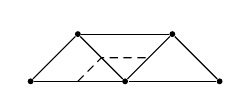
\begin{tikzpicture}[scale=.6,every node/.style={circle,fill,inner sep=.75pt}]
  \path (0,0) node (a)   {}
                 (-2,0) node (b)   {} edge (a)
             (-1,1) node (c)   {} edge (a) edge (b)
             (1,1) node (d)   {} edge (a) edge (c)
             (2,0) node (e)   {} edge (a) edge (d)
          (-1.5,.5) node[coordinate,label=above left:\small] (T0) {}
          (0,1) node[coordinate,label=above:\small] (T1) {}
          (1.5,.5) node[coordinate,label=above right:\small] (T2) {};
  \draw[densely dashed] (-1,0) -- (-.5,.5) -- (.5,.5);
 \end{tikzpicture}
\qquad\qquad
 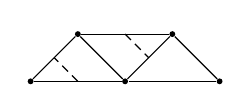
\begin{tikzpicture}[scale=.6,every node/.style={circle,fill,inner sep=.75pt}]
  \path (0,0) node (a)   {}
                 (-2,0) node (b)   {} edge (a)
             (-1,1) node (c)   {} edge (a) edge (b)
             (1,1) node (d)   {} edge (a) edge (c)
             (2,0) node (e)   {} edge (a) edge (d)
          (-1.5,.5) node[coordinate,label=above left:\small] (T0) {}
          (0,1) node[coordinate,label=above:\small] (T1) {}
          (1.5,.5) node[coordinate,label=above right:\small] (T2) {};
  \draw[densely dashed] (-1,0) -- (-1.5,.5) (0,1) -- (.5,.5);
 \end{tikzpicture}
\caption{ is a group of linking triangles in a chain.
In any case,  can be drawn so that  crosses also the common edge of  and~.}
\label{fig:firstcross}
\end{figure}


\begin{lemma}\label{lem:fold2}
Let  be a 2-tree with  vertices and  linking triangles.
The procedure \fold2{G,\ell} produces a folded drawing
of  with more than  interposed vertices lying on the line~.
\end{lemma}

\begin{proof}
Denote the number of interposed vertices on  by .
The rules of \foldn2 for drawing chains ensure that
 is equal to the number of complete groups of linking triangles in .
Let  denote the number of chains in , which is the trivial upper bound
for the number of incomplete groups. We, therefore, have

By Lemma \ref{lem:chains}, we also have

It follows that , yielding the desired bound.
\end{proof}



\subsection{The rest of the proof}

Notice that the rules of \foldn1 and \foldn2 are coherent
and we can consider a hybrid procedure \fold{1+2}{G,\ell}.
This procedure aims at locating on  as many leaf vertices
as \fold{1}{G,\ell} does and as many interposed vertices as
\fold{2}{G,\ell} does.
The latter goal is achieved by adopting the instructions of \foldn2
for drawing chains. The former goal is achieved, like \foldn1, 
by randomization. In order to ensure that, with nonzero probability,
at least  vertices are put on ,
we need to fulfill the following condition:
\begin{enumerate}
\item[(*)]
if  is neither a leaf triangle nor a linking triangle in a complete group, then
each edge of  is crossed by  with probability~.
\end{enumerate}
The exceptional treatment of linking triangles
does not decrease the chances of any leaf vertex to be put on .
Indeed, either a linking triangle  has no leaf triangle in the neighborhood or
 is the end triangle in a chain neighboring with a leaf triangle .
In the latter case the common edge of  and  can be crossed, see Fig.~\ref{fig:groups}
(hence, the leaf vertex of  will be put on~).

However, some care is needed to fulfill Condition (*)
on leaving the last complete group  in a chain. Notice that
in each of the four cases shown in Fig.~\ref{fig:groups} we have two choices for an edge of the
end triangle  that will be crossed by . We make this choice
at random, with probability distribution shown in Fig.~\ref{fig:leaving}.
This ensures (*) for the next neighbor  of~.

\begin{figure}
\centering
 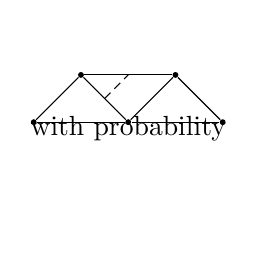
\begin{tikzpicture}[scale=.6,every node/.style={circle,fill,inner sep=.75pt}]
  \path (0,0) node (a)   {}
                 (-2,0) node (b)   {} edge (a)
             (-1,1) node (c)   {} edge (a) edge (b)
             (1,1) node (d)   {} edge (a) edge (c)
             (2,0) node (e)   {} edge (a) edge (d)
          (-1.5,.5) node[coordinate,label=above left:\small] (T0) {}
          (0,1) node[coordinate,label=above:\small] (T1) {}
          (1.5,.5) node[coordinate,label=above right:\small] (T2) {};
  \path (0,2) node[coordinate,label=below:with probability ] (x)   {};
  \draw[densely dashed] (-.5,.5) -- (0,1);
 \end{tikzpicture}
\qquad\qquad
 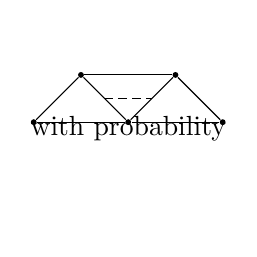
\begin{tikzpicture}[scale=.6,every node/.style={circle,fill,inner sep=.75pt}]
  \path (0,0) node (a)   {}
                 (-2,0) node (b)   {} edge (a)
             (-1,1) node (c)   {} edge (a) edge (b)
             (1,1) node (d)   {} edge (a) edge (c)
             (2,0) node (e)   {} edge (a) edge (d)
          (-1.5,.5) node[coordinate,label=above left:\small] (T0) {}
          (0,1) node[coordinate,label=above:\small] (T1) {}
          (1.5,.5) node[coordinate,label=above right:\small] (T2) {};
  \path (0,2) node[coordinate,label=below:with probability ] (x)   {};
  \draw[densely dashed] (-.5,.5) -- (.5,.5);
 \end{tikzpicture}\\label{eq:bound12}
\frac23\,t_1+t_2-\frac45\,n
\label{eq:t1t2}
4t_1+t_2\ge t+3.
-10mm]\mbox{}
\caption{Proof of Lemma \protect\ref{lem:t1t2} (illustrative fragments of ).}
\label{fig:proofcases}
\end{figure}

An example in Fig.~\ref{fig:4best} shows that the factor of 4 in the bound
\refeq{t1t2} cannot be improved.

\begin{figure}[b]
\centering
 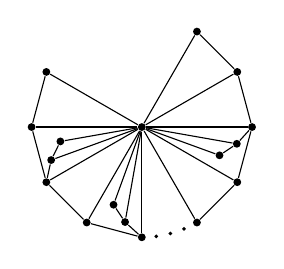
\begin{tikzpicture}[every node/.style={circle,fill,inner sep=1pt}]
  \path[scale=.7] (0,0) node (o)   {}
                (150:2cm) node (a)   {} edge (o)
                (180:2cm) node (b)   {} edge (o) edge (a)
                (-150:2cm) node (c)   {} edge (o) edge (b)
                (-160:1.75cm) node (c1)   {} edge (o) edge (c)
                (-170:1.5cm) node (c2)   {} edge (o) edge (c1)
                (-120:2cm) node (d)   {} edge (o) edge (c)
                (-90:2cm) node (e)   {} edge (o) edge (d)
                (-100:1.75cm) node (e1)   {} edge (o) edge (e)
                (-110:1.5cm) node (e2)   {} edge (o) edge (e1)
                (-60:2cm) node (f)   {} edge (o)
                (-82.5:2cm) node[inner sep=.5pt] (f1)   {}
                (-75:2cm) node[inner sep=.5pt] (f2)   {}
                (-67.5:2cm) node[inner sep=.5pt] (f3)   {}
                (-30:2cm) node (g)   {} edge (o) edge (f)
                (0:2cm) node (h)   {} edge (o) edge (g)
                (-10:1.75cm) node (h1)   {} edge (o) edge (h)
                (-20:1.5cm) node (h2)   {} edge (o) edge (h1)
                (30:2cm) node (i)   {} edge (o) edge (h)
                (60:2cm) node (j)   {} edge (o) edge (i);
 \end{tikzpicture}
\caption{A 2-tree with   triangles, for which  and 
(the parameter  can take an arbitrary value).}
\label{fig:4best}
\end{figure}


Turning back to the proof of Theorem \ref{thm:2trees}, suppose first that .
In this case the bound \refeq{bound12} has no advantage upon the performance of
\fold1{G,\ell}, that puts at least  vertices on .
By Lemma \ref{lem:t1t2}, we then have ,
and hence  passes trough more than  vertices.
If , the procedure \foldn{1+2} is preferable and yields

collinear vertices. The proof is complete.





\section{Questions and comments}\label{s:open}
\mbox{}

\que
How far or close are parameters  and ?
It seems that a priori we even cannot exclude equality.
To clarify this question, it would be helpful to (dis)prove that every collinear set 
in any straight line drawing is free.


\que
We constructed examples of graphs with 
for a graph-theoretic constant , for which it is known that
. Are there graphs with ?
If so, this could be considered a strengthening of the examples of graphs
with  given in \cite{Bose,merged,KPRSV}.
Are there graphs with, at least, ? If not,
by Theorem \ref{thm:fixfree} this would lead to an improvement of 
Bose et al.'s bound~\refeq{bose}.

\que
By Theorem \ref{thm:2trees}, we have 
for any graph  with tree-width no more than 2.
One can also show that for Halin graphs, whose tree-width can attain 3,
we have .
For which other classes of graphs do we have 
or, at least, ? In particular, is  linear
for 2-outerplanar graphs? These graphs have tree-width at most 5,
and one can extend this question to planar graphs with tree-width bounded by a small
constant . Corollary \ref{cor:btw} gives a negative answer if  is sufficiently large.
Furthermore, what about planar graphs with bounded vertex degrees?
Note that the graphs constructed in the proof of Theorem \ref{thm:lin}
have vertices with degree more than  for some .

\que
In a recent paper \cite{CanoTU11},
Cano, T\'oth, and Urrutia improve the upper bound \refeq{fixupper}
to a bound of . Similarly to our proof of Theorem \ref{thm:lin},
their construction also uses iterative refinement
of faces of a planar triangulation.
It follows that our lower bound of  in Corollary \ref{cor:2trees} 
cannot be extended to any class of planar graphs with bounded tree-width,
even to planar graphs of tree-width 8. If such extension is possible
for tree-width 3,4,\ldots is a natural open problem.

\que
Whether or not  is an intriguing question.
Similarly to \refeq{fixfixl}, one can prove that ,
where  with the minimization over collinear .
Thus, the question is actually whether or not
 has the same value for all collinear .
A similar question for  is also open; it is posed in \cite[Problem 6.5]{KPRSV}.
\edit{
These questions have a strong flavour of \emph{morphing} issues, see, e.g., \cite{}.
}

\que
It is also natural to consider , where the minimization goes over
all  in general position. Can one extend our upper bound  to show
that  for infinitely many ?

\hide{
\que
Since grid graphs are almost layered, we have for them 
where .
How tight is this lower bound?
From \cite[Corollary 4.1]{Cib} we know that .
}

\que
By slightly modifying the proof of Lemma \ref{lem:Gk}.2,
one can show that .
It follows that, for any cubic polyhedral graph ,
there exists a sequence of cubic polyhedral graph 
such that .
This readily implies two properties of the shortness exponent
for cubic polyhedral graphs, that seem to be unnoticed so far.
First,  over all
cubic polyhedral . Second,  cannot be attained
by the fraction  for any particular~.
It is interesting if this holds true for other families of graphs.

\begin{thebibliography}{10}


\bibitem{BilinskiJMY11}
M.~Bilinski, B.~Jackson, J.~Ma, X.~Yu.
\newblock
Circumference of 3-connected claw-free graphs and large Eulerian subgraphs 
of 3-edge-connected graphs.
\newblock
{\em Journal of Combinatorial Theory, Series B} 101(4):214--236 (2011).


\bibitem{Bodlaender98}
H.L.~Bodlaender.
\newblock
A partial -arboretum of graphs with bounded treewidth.
\newblock
{\it Theoretical Computer Science} 209(1-2):1--45 (1998).


\bibitem{Bose}
P.~Bose, V.~Dujmovic, F.~Hurtado, S.~Langerman, P.~Morin, D.R.~Wood.
\newblock
A polynomial bound for untangling geometric planar graphs. 
\newblock
{\em Discrete and Computational Geometry} 42(4):570--585 (2009).

\bibitem{CanoTU11}
J.~Cano, C.D.~T\'oth, J.~Urrutia.
\newblock
Upper bound constructions for untangling planar geometric graphs.
\newblock
Proc.\ of the 19-th Int.\ Symp.\ on {\em Graph Drawing, 2011},
to appear.

\bibitem{Cib}
J.~Cibulka.
\newblock
Untangling polygons and graphs.
\newblock
{\em Discrete and Computational Geometry} 43(2):402--411 (2010).

\bibitem{FelsnerLW03}
S.~Felsner, G.~Liotta, S.K.~Wismath.
\newblock
Straight-line drawings on restricted integer grids in two and three dimensions. 
\newblock
{\em J.~Graph Algorithms Appl.} 7(4):363--398 (2003).


\bibitem{FlajoletN99}
P.~Flajolet, M.~Noy.
\newblock Analytic combinatorics of non-crossing configurations.
\newblock {\em Discrete Mathematics}, 204(1-3):203--229, 1999.

\bibitem{GarciaHHTV09}
A.~Garc\'{\i}a, F.~Hurtado, C.~Huemer, J.~Tejel, P.~Valtr.
\newblock On triconnected and cubic plane graphs on given point sets.
\newblock {\em Comput. Geom.} 42(9):913--922, 2009.

\bibitem{GimenezN09}
O.~Gim\'enez, M.~Noy.
\newblock {Counting planar graphs and related families of graphs.}
\newblock In: {\it Surveys in combinatorics 2009.}
Cambridge: Cambridge University Press, pages 169--210 (2009).

\bibitem{merged}
X.~Goaoc, J.~Kratochv\'{\i}l, Y.~Okamoto, C.S.~Shin, A.~Spillner, A.~Wolff.
\newblock
Untangling a planar graph.
\newblock
{\it Discrete and Computational Geometry\/} 42(4):542--569 (2009).

\bibitem{GritzmannMPP91}
P.~Gritzmann, B.~Mohar, J.~Pach, R.~Pollack.
\newblock Embedding a planar triangulation with vertices at specified points.
\newblock {\em American Mathematical Monthly} 98(2):165--166, 1991.

\bibitem{Gru}
B.~Gr\"unbaum.
\newblock
How to cut all edges of a polytope?
\newblock
{\it The American Mathematical Monthly} 79(8):890--895 (1972).

\bibitem{GWa}
B.~Gr\"unbaum, H.~Walther.
\newblock
Shortness exponents of families of graphs.
\newblock
{\it J.\ Combin.\ Theory A} 14:364--385 (1973).

\bibitem{KPRSV}
M.~Kang, O.~Pikhurko, A.~Ravsky, M.~Schacht, O.~Verbitsky.
\newblock
Untangling planar graphs from a specified vertex position
--- Hard cases.
\newblock
{\it Discrete Applied Mathematics} 159:789--799 (2011).



\bibitem{PTa}
J.~Pach, G.~Tardos.
\newblock
Untangling a polygon. 
\newblock
{\it Discrete and Computational Geometry\/} 28:585--592 (2002).

\bibitem{Ver}
O.~Verbitsky.
\newblock
On the obfuscation complexity of planar graphs.
\newblock
{\it Theoretical Computer Science\/} 396(1--3):294--300 (2008).

\end{thebibliography}

\end{document}
